%\documentclass[compress,dvips,xcolor=table]{beamer}
\usepackage{etex}
%\documentclass{article}
%\usepackage{beamerarticle}
%\usepackage{pstricks,pst-node} % PSTricks package
%\usepackage[turkish]{babel}
\usepackage[utf8]{inputenc}
\usepackage{listings}
\usepackage{array}
\usepackage{multicol}
\usepackage{tikz}
\usetikzlibrary{trees,automata}
%\includeonlyframes{current}

\def\circtxt#1{$\mathalpha \bigcirc \mkern-13mu \mathtt #1$}

\mode<article>
{
  \usepackage{fullpage}
  \usepackage{pgf}
  \usepackage{hyperref}
}

\mode<presentation>
{
  \usetheme{metuceng}

%  \setbeamercovered{transparent}
}


\title{Programming Language Concepts}
\subtitle{Logic Programming Paradigm}
\author{Onur Tolga Şehitoğlu}
\institute[ODTÜ]{Bilgisayar Mühendisliği}
\subject{Logic Programming}
\date{}
	\titlegraphic{\insertmetutitle\insertlicense}


\begin{document}
\lstset{language=Prolog,
        basicstyle=\scriptsize\ttfamily,
        keywordstyle=\color{blue!50!black}\bfseries,
        identifierstyle=\color{blue!60!green}\sffamily,
        stringstyle=\color{red!70!green}\ttfamily,
	commentstyle=\color{blue!30!white}\itshape,
        showstringspaces=true}
\setbeamercolor{hexample}{bg=green!5!white,fg=black}%
\setbeamercolor{cexample}{bg=blue!5!white,fg=black}%
\setbeamercolor{pexample}{bg=orange!5!white,fg=black}%
\setbeamercolor{oexample}{bg=violet!5!white,fg=black}%

 \frame[plain]{\maketitle}
 \begin{frame}
 \frametitle{Outline}
 \begin{multicols}{2}
 \tableofcontents
 \end{multicols}
 \end{frame}

\section{Introduction}
\begin{frame}
\frametitle{Logic Programming Paradigm}
\begin{itemize}
\item Based on logic and \structure{declarative programming}
\item 60's and early 70's 
\item Prolog (\textbf{Pro}gramming in \textbf{log}ic, 1972) is
	the most well known representative of the paradigm.
\item Prolog is based on \structure{Horn clauses} and 
	\structure{SLD resolution} 
\item Mostly developed in \structure{fifth generation computer systems
	project}
\item Specially designed for theorem proof and artificial intelligence but
	allows general purpose computation.
\item Some other languages in paradigm: ALF, Frill, Gödel, Mercury, Oz,
Ciao, $\lambda$Prolog, datalog, and CLP languages
\end{itemize}
\end{frame}

\begin{frame}
\frametitle{Constraint Logic Programming}
\begin{itemize}
\item
Clause: disjunction of universally quantified literals,
\[ \forall(L_1 \vee L_2 \vee ... \vee L_n) \]
\item
A logic program clause is a clause with exactly one
positive literal
\[ \begin{array}{l}
   \forall(A \vee \neg A_1 \vee \neg A_2 ... \vee \neg A_n) \equiv \\
   \forall(A \Leftarrow A_1 \wedge A_2 ... \wedge  A_n) 
\end{array}\] 

\item
A goal clause: no positive literal
\[ \forall(\neg A_1 \vee \neg A_2 ... \vee \neg A_n) \]

\item
Proof by refutation, try to unsatisfy the clauses with
a goal clause $G$. Find $\exists(G)$.
\item
Linear resolution for definite programs with constraints and
selected atom.
\end{itemize}
\end{frame}

\defverbatim[colored]\codefamily{
\begin{lstlisting}[language=Prolog,escapechar=\#]
father(ahmet,ayse).
father(hasan,ahmet).
mother(fatma,ayse).
mother(hatice,fatma).
parent(X,Y) :- father(X,Y).
parent(X,Y) :- mother(X,Y).
grandparent(X,Y) :- parent(X,Z),parent(Z,Y).
\end{lstlisting}}
\begin{frame}
\frametitle{What does Prolog look like?}
\begin{beamercolorbox}{oexample}
\codefamily
\end{beamercolorbox}

\end{frame}

\section{Prolog basics}
\begin{frame}
\begin{itemize}
\item CLP on first order terms. (Horn clauses).
\item \structure{Unification}. Bidirectional.
\item \structure{Backtracking}. Proof search based on trial of all matching
	clauses.
\end{itemize}
\end{frame}

\section{Prolog Terms}
\begin{frame}[fragile]
\frametitle{Prolog Terms}
\begin{itemize}
\item Every valid phrase in prolog is a \structure{Term} and instead of strict type checking, \structure{unification} is used. A term can be one of the following:
\item Atoms:
	\begin{enumerate}
	\item Strings with starting with a small letter and followed by any letter, digit and \lstinline!_!.
		\lstinline{[a-z][a-zA-Z_0-9]*}
	\item Strings consisting of only punctuation symbols as:\\
        \lstinline{[+-*/\^<>=~:.?@#$!&]+}
\item \lstinline@[],  {},  ;, !@ are only treated as atoms in these  forms (alone and only
spaces in between).
	\item Any string enclosed in single or back quotes. Quotes are not part of the atom.
	\end{enumerate}
\item Numbers
    \begin{enumerate}
    \item Any integer \lstinline![0-9]+!
    \item Any floating point value \lstinline![0-9]+.[0-9]+!
    \item Any scientific notation value \lstinline![0-9]+.[0-9]+e[0-9]+!
    \end{enumerate}
\end{itemize}
\end{frame}
\begin{frame}
\begin{itemize}
\item Variables:
	\begin{enumerate}
	\item Strings with starting with a capital letter or {\tt \_} and consist of
		\lstinline![_A-Z][a-zA-Z_0-9]*!
	\item {\tt \_} alone is the universal match symbol. Not variable
	\end{enumerate}
\item Structures:
	\begin{itemize}
	\item starts with an \structure{atom} head. No number, no variable
	\item has one or more arguments enclosed in paranthesis, separated by comma
	\item no space between structure head and paranthesis.
    \item arguments can be any valid prolog term, including other structures.
	\end{itemize}
\end{itemize}
\end{frame}

\def\OK{\only<2->{\color{green!50!black}$\surd$}}

\begin{frame}[fragile]
\scriptsize

\rowcolors[]{2}{blue!10!white}{blue!5!white}
\begin{tabular}{|l|c|c|c|c|c|}\hline
\rowcolor{blue!40!white}
Term  & Atom & Num. & Var. & Struct. & not a term \\ \hline
\lstinline!hELLO!  & \OK    &       &       &       	&	\\ \hline
\lstinline!Hello!  &     &       & \OK      &       	&	\\ \hline
\lstinline!_abc!  &     &       &   \OK     &       	&	\\ \hline
\lstinline!'A and B'!  &  \OK    &       &       &       	&	\\ \hline
\lstinline!"hello"! &   &   &   &  \OK  &   \\ \hline
\lstinline!:->>!   &  \OK    &       &       &       	&	\\ \hline
\lstinline!:-P!    &     &       &       &       	&\OK 	\\ \hline
\lstinline!__!  &     &       &  \OK      &       	&	\\ \hline
\lstinline!1e1!  &     &  \OK      &       &       	& 	\\ \hline
\lstinline!1.0e1!  &     &   \OK     &       &       	&	\\ \hline
\lstinline!0.2!  &     &  \OK      &       &       	&	\\ \hline
\lstinline!.2!  &     &       &       &       	&\OK 	\\ \hline
\lstinline!3.!  &     &       &       &       	&\OK 	\\ \hline
\lstinline!0000123!  &     &   \OK    &       &       	& 	\\ \hline
\lstinline!x(4)!  &     &       &       &  \OK      	&	\\ \hline
\lstinline!++(a,b)!  &     &       &       & \OK       	&	\\ \hline
\lstinline!R(3)!  &     &       &       &       	&	\OK \\ \hline
\lstinline!2(4)!  &     &       &       &       	&\OK 	\\ \hline
\lstinline!a(a(a,a(a(a(a)))))!  &     &       &   \OK     &       	&	\\ \hline
\lstinline!a(X,Y,.(X),2,3)!  &     &       &       &     \OK   	&	\\ \hline
\end{tabular}
\end{frame}

\begin{frame}[fragile]
\frametitle{Syntax Elements}
\begin{itemize}
\item A Prolog program consists of \structure{clauses} or \structure{predicates}.
\item \structure{Unit clauses} are structure or atom terms followed by a dot.\\
    \lstinline!father(ayse, ahmet).!
\item Unit clauses are considered as facts, no implication.
\item Non-unit clauses consists of a \structure{head clause} and a \structure{body}\\
    \lstinline!grand(X, Y) :- parent(X,Z), parent(Z,X).!
\item In order to prove head clause, body should be proven.
\item Body consist of structures seperated by comma, semi-colon and optionally combined with
parantheses.\\
    \lstinline{uncle(X,Y) :- (brother(X,Z),father(Z,Y)) ; (brother(X,Z), mother(Z,Y)).}
\item Comma stands for conjunction ($\wedge$), semicolon stands for disjunction ($\vee$).
\item Structures in the body are \structure{goal clauses} to be proven.
\end{itemize}
\end{frame}

\begin{frame}
\frametitle{Prolog Lists}
\begin{itemize}
\item \lstinline![1,2,3]! is parsed and interpreted as \lstinline!.(1,.(2,.(3,[])))!
\item \lstinline![Head | Tail]! form is interpreted as \lstinline!.(Head , Tail)!
\item \lstinline![]! denotes empty list
\item \lstinline![1,2,3 | R]! is interpreted as \lstinline!.(1, .(2, .(3, R)))!
\item strings in double quotes like \lstinline!"abc"! are interpreted as
list of ASCII numbers as \lstinline![97, 98, 99]!.
\item As Prolog structures can contain arbitrary terms,  lists are heteregenous as 
\lstinline![1, 2.1, a(b,c), [a,b,c],"hello"]! is a valid list.
\end{itemize}
\end{frame}

\section{Unification}
\begin{frame}[fragile]
\frametitle{Unification}
\begin{itemize}
\item In functional languages, caller arguments are pattern-matched
against the function definition. This operation is also
called \structure{unification}.  All constructors and values in caller
are matched against the patterns in the definition. The variables in
definition are \structure{instantiated} with the values in the caller.
\item Unification in Prolog is bi-directional. Both the defining clause and goal clause
have variables instantiated.\\
\lstinline!same(X,X).!\\
goal: \lstinline!same(ali,Y).!\\
\lstinline!X = ali, Y = X, Y = ali!
\item Result of a unification can result in some variable instantiations as:\\
\lstinline!X = ali, Y = ali! $\Rightarrow$ \lstinline!true!
\end{itemize}
\end{frame}

\begin{frame}
\frametitle{Unification of Terms}
unification of $x$ and $y$ is successfull, $x = y$ $\Leftrightarrow$ \\
\begin{enumerate}[<+->]
\item $x$ is atom or number and $y$ is the same atom or number
\item $x$, and $y$ are structures with \structure{same arity} $n$,\\
 $x = h_x(x_1,x_2, ..., x_n)$, $y = h_y(y_1, y_2, ..., y_n)$ and\\
$h_x = h_y$ and $\forall x_i = y_i, \; i = 1, ... n$. Head and all coressponding
elements are unified.
\item If $x$ is a variable and $x = y$ is compatible with the current set of instantiations,
unification is successfull with $x = y$ is added to current set of instantiations.
\item Otherwise, unification fails.
\end{enumerate}
\end{frame}

\begin{frame}[fragile]
\scriptsize
\rowcolors[]{2}{blue!5!white}{blue!10!white}
\begin{tabular}{lp{.55\textwidth}}\rowcolor{blue!5!white}
\lstinline!a = b!	   & false  \\[1em]
\lstinline!'abc' = abc!	 & true \\[1em]
\lstinline!X = 12!	 & true $\Leftarrow$ X=12 \\[1em]
\lstinline!a(1,X) = a(Y,2)!	 & true $\Leftarrow$ X=2, Y=1 \\[1em]
\lstinline!a(1,X) = a(Y,Y)!	 & true $\Leftarrow$ X=Y=1 \\[1em]
\lstinline!a(1,X,X) = a(Y,Y,2)!	 & false (Y=1, X=Y, X=2) \\[1em]
\lstinline!a(1,_) = a(1)!	 & false (different arities)\\[1em]
\lstinline!X = a(X)!	 & true $\Leftarrow$ X = a(X) (cannot display but succesfull) \\[1em]
\lstinline!a(c(X,d),c(a,Y),X) = a(Y,Z,t)! & true $\Leftarrow$ X = t, Y = c(t,d) , Z = c(a,c(t,d))\\[1em]
\lstinline!a(c(X,d),c(a,Y)) = a(Y,X)! & true $\Leftarrow$ X = c(a,Y), Y = c(X,d)\\[1em]
\end{tabular}

\end{frame}

\begin{frame}
\frametitle{Prolog Program}
\begin{itemize}
\item A Prolog program can be written by putting all alternatives as a seperate
head clause with same name and arity.
\item You define \structure{relations} instead of functions returning a value.
\item For example, not a membership test function but a \structure{member relation}.
\item Membership relation for a list can be defined verbally as:\\
``$x$ is member of list $lst$ if either $x$ is the first element of the $lst$ or
it is the member of the remaining list''
\item Each alternative is another \lstinline!member(X,LST)! clause.\\
    \lstinline!member(X, [First | Remaining]) :- X = First.!\\
    \lstinline!member(X, [First | Remaining]) :- member(X, Remaining).!\\
\item Shorter form:\\
    \lstinline!member(X, [X | _ ]).!\\
    \lstinline!member(X, [_ | Remaining]) :- member(X, Remaining).!\\
\end{itemize}
\end{frame}

\begin{frame}[fragile]
\frametitle{Prolog Interpreter}
\begin{itemize}
\item \structure{Gnu Prolog} or \structure{Sicstus Prolog} are free alternatives.
\item entering `\lstinline![filename].!' in interpreter loads the clauses from \texttt{filename.pl}.
\item `\lstinline!?- !' prompt asks user to enter goal clauses like:\\
\lstinline!?- member(b, [a,b,c]).!
\item Prolog checks if this goal can be proven with the current program and replies
\structure{yes}, \structure{no}
\item If there are alternatives, it prompts \structure{true ?} and asks for continuation.
pressing enter will terminate, \structure{;} will try other alternatives.
\end{itemize}
\end{frame}

\begin{frame}[fragile]
\begin{beamercolorbox}{oexample}
\begin{lstlisting}
~$ swipl
Welcome to SWI-Prolog (Multi-threaded, 64 bits, Version 7.2.3)
...
Please visit http://www.swi-prolog.org for details.

?- [testmember].          % load testmember.pl
true.
?- member(b,[a,b,c]).
true                      % hit enter 
?- member(d, [a,b,c]).
false.
?- member(b,[a,b,c]).
true ;                    % hit ; , try alternatives
false.                    % no other alternatives true
?- member(b,[a,b,b]).     
true ;                    % hit ; , try alternatives
true ;                    % one more alternative, no other
false.
?- member(X,[a,b,c]).     % ask who is member of [a,b,c]?
X = a ;
X = b ;
X = c ;
false.
\end{lstlisting}
\end{beamercolorbox}
\end{frame}

\section{Backtracking}
\begin{frame}
\frametitle{Backtracking}
\begin{itemize}
\item Backtracking is the search procedure of Prolog and makes it a universal
programming language.
\item Each alternative head clause that can be \structure{unified} with goal clause
is a \structure{backtracking} point.
\item similarly each operand of `\texttt{;}' is a backtracking point.
\item Prolog saves the current state in backtracking points. On failure,
tries the next backtraking branch.
\item On success, if user hits `\texttt{;}' in prompt, it resumes
search from the next backtracking point.
\end{itemize}
\end{frame}
\def\BT{\textcolor{red!50!black}{\small\bf ;}}

\begin{frame}[fragile]
    \lstinline[basicstyle=\tiny\ttfamily]!member(X, [X | _ ]).!\\
    \lstinline[basicstyle=\tiny\ttfamily]!member(X, [_ | Rem]) :- member(X, Rem).!\\[1em]
\tiny
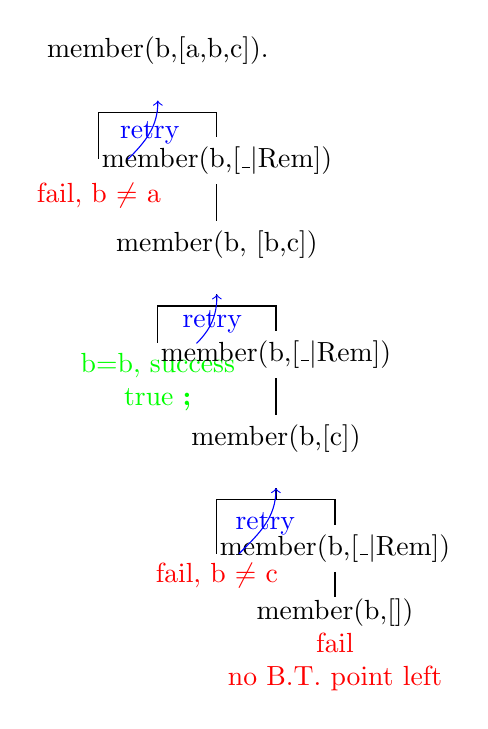
\begin{tikzpicture} [edge from parent fork down,level distance=3.5em,align=center]
\node (bt1) {member(b,[a,b,c]).\\ \BT } 
    child { node [red,yshift=-1em] (f1) {\\fail, b $\not =$ a} } 
    child { node {member(b,[\_$\mid$Rem])}
       child { node (bt2) {member(b, [b,c]) \\ \BT }
           child { node [yshift=-1em,green] (s2) { b=b, success \\ {true \bf ;} }}
           child { node {member(b,[\_$\mid$Rem])} 
               child { node (bt3) {member(b,[c])  \\ \BT} 
                    child { node [red,yshift=-1em] (f3) {fail, b $\not =$ c}}
                    child { node {member(b,[\_$\mid$Rem])}
                        child { node {member(b,[])\\ \textcolor{red}{fail}\\
                            \textcolor{red}{no B.T. point left}} }
                    }
                }
           }
       }
   };
\draw [->,blue] (f1) to [out=45,in=270] node {retry} (bt1.south);
\draw [->,blue] (s2) to [out=45,in=270] node {retry} (bt2.south);
\draw [->,blue] (f3) to [out=45,in=270] node {retry} (bt3.south);
\end{tikzpicture}
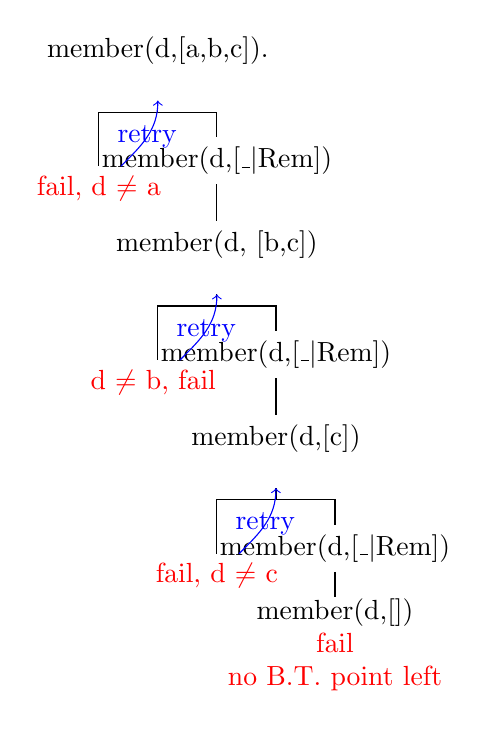
\begin{tikzpicture} [edge from parent fork down,level distance=3.5em,align=center]
\node (bt1) {member(d,[a,b,c]).\\ \BT } 
    child { node [red,yshift=-1em] (f1) {fail, d $\not =$ a} } 
    child { node {member(d,[\_$\mid$Rem])}
       child  { node (bt2) {member(d, [b,c]) \\ \BT }
           child { node [yshift=-1em,red] (f2) { d $\not =$ b, fail }}
           child { node {member(d,[\_$\mid$Rem])} 
               child { node (bt3) {member(d,[c]) \\ \BT} 
                    child { node [red,yshift=-1em] (f3) {fail, d $\not =$ c}}
                    child { node {member(d,[\_$\mid$Rem])}
                        child { node {member(d,[])\\ \textcolor{red}{fail}\\
                                      \textcolor{red}{no B.T. point left}} }
                    }
                }
           }
       }
   };
\draw [->,blue] (f1) to [out=45,in=270] node {retry} (bt1.south);
\draw [->,blue] (f2) to [out=45,in=270] node {retry} (bt2.south);
\draw [->,blue] (f3) to [out=45,in=270] node {retry} (bt3.south);
\end{tikzpicture}
\end{frame}

\begin{frame}[fragile]
    \lstinline[basicstyle=\tiny\ttfamily]!member(X, [X | _ ]).!\\
    \lstinline[basicstyle=\tiny\ttfamily]!member(X, [_ | Rem]) :- member(X, Rem).!\\[1em]
\tiny
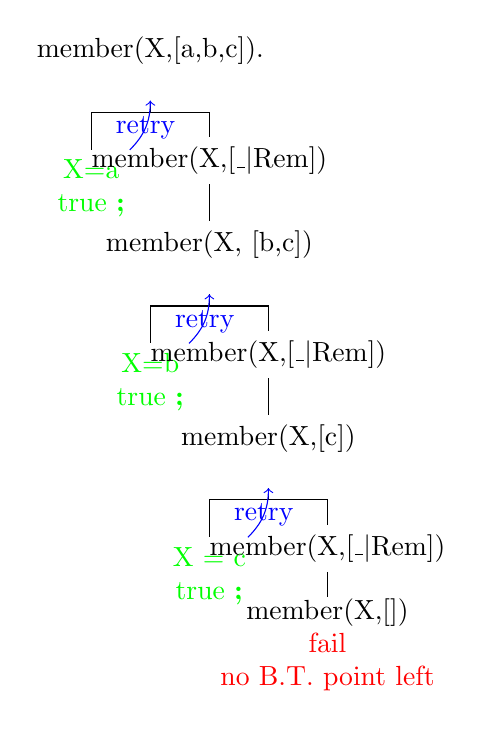
\begin{tikzpicture} [edge from parent fork down,level distance=3.5em,align=center]
\node (bt1) {member(X,[a,b,c]).\\ \BT } 
    child { node [green,yshift=-1em] (s1) {X=a \\ true \bf ;} } 
    child { node {member(X,[\_$\mid$Rem])}
       child { node (bt2) {member(X, [b,c]) \\ \BT }
           child { node [yshift=-1em,green] (s2) { X=b \\ true \bf ; }}
           child { node {member(X,[\_$\mid$Rem])} 
               child { node (bt3) {member(X,[c])  \\ \BT} 
                    child { node [green,yshift=-1em] (s3) {X = c \\ true \bf ;}}
                    child { node {member(X,[\_$\mid$Rem])}
                        child { node {member(X,[])\\ \textcolor{red}{fail}\\
                            \textcolor{red}{no B.T. point left}} }
                    }
                }
           }
       }
   };
\draw [->,blue] (s1) to [out=45,in=270] node {retry} (bt1.south);
\draw [->,blue] (s2) to [out=45,in=270] node {retry} (bt2.south);
\draw [->,blue] (s3) to [out=45,in=270] node {retry} (bt3.south);
\end{tikzpicture}
\end{frame}

\begin{frame}[fragile]
    \begin{tabular}{lll}
    \lstinline[basicstyle=\tiny\ttfamily]!mother(fatma,veli).! &
    \lstinline[basicstyle=\tiny\ttfamily]!father(ali, hasan).! &
    \lstinline[basicstyle=\tiny\ttfamily]!parent(X,Y) :- mother(X,Y).! \\
    \lstinline[basicstyle=\tiny\ttfamily]!mother(ayse, ali).! &
    \lstinline[basicstyle=\tiny\ttfamily]!father(hasan, veli).! &
    \lstinline[basicstyle=\tiny\ttfamily]!parent(X,Y) :- father(X,Y).! \\
    \multicolumn{3}{l}{ \lstinline[basicstyle=\tiny\ttfamily]!gp(X,Y) :- parent(X,Z), parent(Z,Y).!} \\
    \end{tabular} \\
\tiny
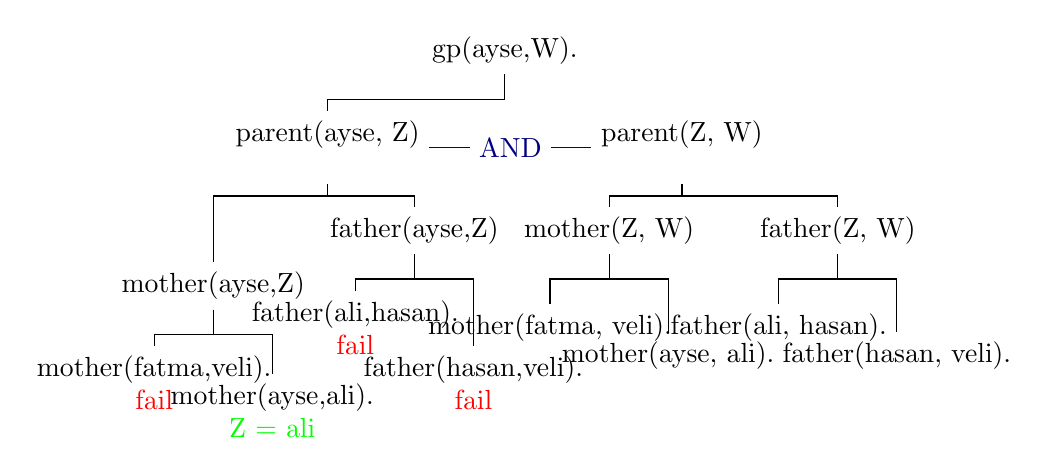
\begin{tikzpicture} [edge from parent fork down,level distance=3.5em,align=center] 
\node (bt1) {gp(ayse,W).}
    child { node (par1) {parent(ayse, Z) \\ \BT}
              child { node [xshift=-2em,yshift=-1.5em]  {mother(ayse,Z)}
                        child { node {mother(fatma,veli). \\ \textcolor{red}{fail}} }
                        child { node [yshift=-1em] {mother(ayse,ali).\\ \textcolor{green}{Z = ali}}}
              }
              child { node [yshift=.5em, xshift=1em] {father(ayse,Z)}
                        child { node {father(ali,hasan). \\ \textcolor{red}{fail}}}
                        child { node [yshift=-2em] {father(hasan,veli). \\ \textcolor{red}{fail}}}
              }
          }
    child [missing] { node {}}
    child [missing] { node {}}
    child { node (par2) {parent(Z, W) \\ \BT} edge from parent [draw=none]
              child { node [xshift=-.5em,yshift=.5em] {mother(Z, W)}
                        child { node {mother(fatma, veli).}}
                        child { node [yshift=-1em] {mother(ayse, ali).}}
                    }
              child { node [xshift=3.5em,yshift=.5em] {father(Z, W)}
                        child { node {father(ali, hasan).}}
                        child { node [yshift=-1em] {father(hasan, veli).}}
              }
          };
\draw [-,blue!50!black] (par1) -- node [fill=white] {AND} (par2);
\end{tikzpicture}
\ \\
Only solution from left branch is \lstinline[basicstyle=\tiny\ttfamily]!Z=ali!, applied to right branch. \lstinline[basicstyle=\tiny\ttfamily]!father(ali,hasan)! matches. Result is \lstinline[basicstyle=\tiny\ttfamily]!W = hasan!.
\end{frame}
\begin{frame}[fragile]
    \begin{tabular}{lll}
    \lstinline[basicstyle=\tiny\ttfamily]!mother(fatma,veli).! &
    \lstinline[basicstyle=\tiny\ttfamily]!father(ali, hasan).! &
    \lstinline[basicstyle=\tiny\ttfamily]!parent(X,Y) :- mother(X,Y).! \\
    \lstinline[basicstyle=\tiny\ttfamily]!mother(ayse, ali).! &
    \lstinline[basicstyle=\tiny\ttfamily]!father(hasan, veli).! &
    \lstinline[basicstyle=\tiny\ttfamily]!parent(X,Y) :- father(X,Y).! \\
    \multicolumn{3}{l}{ \lstinline[basicstyle=\tiny\ttfamily]!gp(X,Y) :- parent(X,Z), parent(Z,Y).!} \\
    \end{tabular} \\
\tiny
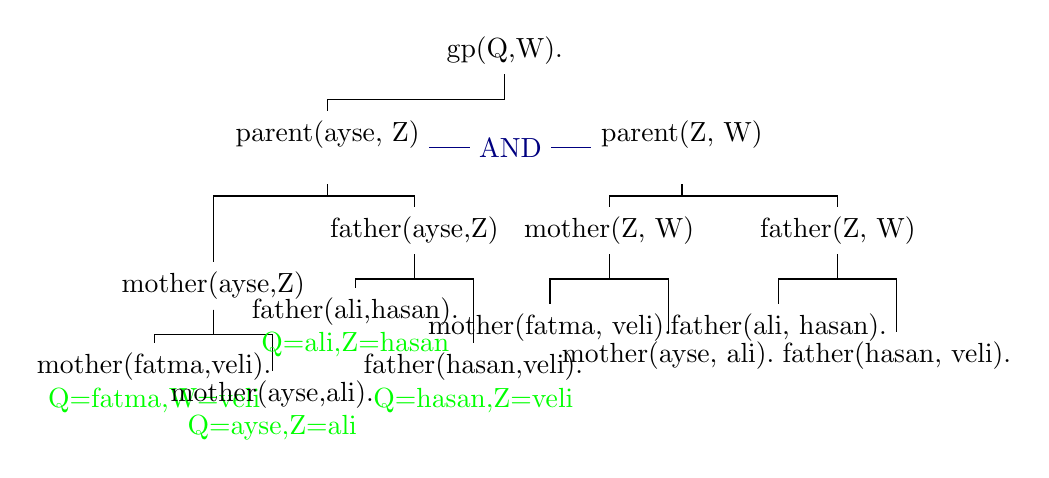
\begin{tikzpicture} [edge from parent fork down,level distance=3.5em,align=center] 
\node (bt1) {gp(Q,W).}
    child { node (par1) {parent(ayse, Z) \\ \BT}
              child { node [xshift=-2em,yshift=-1.5em]  {mother(ayse,Z)}
                        child { node {mother(fatma,veli). \\ \textcolor{green}{Q=fatma,W=veli}} }
                        child { node [yshift=-1em] {mother(ayse,ali).\\ \textcolor{green}{Q=ayse,Z=ali}}}
              }
              child { node [yshift=.5em, xshift=1em] {father(ayse,Z)}
                        child { node {father(ali,hasan). \\ \textcolor{green}{Q=ali,Z=hasan}}}
                        child { node [yshift=-2em] {father(hasan,veli). \\ \textcolor{green}{Q=hasan,Z=veli}}}
              }
          }
    child [missing] { node {}}
    child [missing] { node {}}
    child { node (par2) {parent(Z, W) \\ \BT} edge from parent [draw=none]
              child { node [xshift=-.5em,yshift=.5em] {mother(Z, W)}
                        child { node {mother(fatma, veli).}}
                        child { node [yshift=-1em] {mother(ayse, ali).}}
                    }
              child { node [xshift=3.5em,yshift=.5em] {father(Z, W)}
                        child { node {father(ali, hasan).}}
                        child { node [yshift=-1em] {father(hasan, veli).}}
              }
          };
\draw [-,blue!50!black] (par1) -- node [fill=white] {AND} (par2);
\end{tikzpicture}
\ \\
For each solution in left parent branch it backtracks and test solution from right parent branch,
keeping the instantiated variables. \lstinline[basicstyle=\tiny\ttfamily]!Z=ali! and
\lstinline[basicstyle=\tiny\ttfamily]!Z=hasan! returns success. Results are:
\lstinline[basicstyle=\tiny\ttfamily]!Q=ayse,W=hasan! and
\lstinline[basicstyle=\tiny\ttfamily]!Q=ali,W=veli!
\end{frame}

\section{List Processing}
\begin{frame}[fragile]
\frametitle{List Processing}
\begin{itemize}
\item Appending lists.\\
\begin{beamercolorbox}{oexample}
\begin{lstlisting}[escapeinside=`']
append([], LST, LST).  
append([H | Rem], LST,`\only<2->{\tt [H | Res]}') :- append (Rem, LST, Res).      
\end{lstlisting}
\end{beamercolorbox}
\item \lstinline!append(X,Y,[a,b,c,d])! works as well.
\item Reverse:\\
\begin{beamercolorbox}{oexample}
\begin{lstlisting}[escapeinside=`']
reverse([], []).    % reverse of empty list
reverse([H|Rem],Rev) :- reverse(Rem, RR), `\only<3->{\tt append(RR,[H], Rev)}'.
\end{lstlisting}
\end{beamercolorbox}
\item Efficient reverse:\\
\begin{beamercolorbox}{oexample}
\begin{lstlisting}[escapeinside=`']
reverse2([], L, L).    % no element left, result is stack
reverse2([H | Rem],P, L) :- reverse2(Rem, [H | P], L). % insert on stack
reverse(LST, LSTREV) :- reverse2(LST, [], LSTREV).
\end{lstlisting}
\end{beamercolorbox}
\end{itemize}
\end{frame}

\section{Arithmetical Operations}
\begin{frame}[fragile]
\frametitle{Arithmetical Operations}
\begin{itemize}
\item \lstinline!X =  3 * 5! is equivalent to \lstinline!X = *(3,5)!
    and does not make any calculation.
\item A special operator `\lstinline!is!' evaluates the expressions:\\
\lstinline!X is 3 * 5! will instantiate X to 15.
\item \lstinline!is! requires right handside to be fully instantiated (no variables without a value) and evaluates it, the resulting number is unified with LHS.
\item `\lstinline!2+X is 5!' is equivalent to unification of \lstinline!+(2,X)! to 5, which fails.
\item Comparison operators also evaluate their both operands which should be fully instantiated:\\
\lstinline!<  , > ,  =< , >=, =:= , =\=!
\item Some of the arithmetic operators (in evaluation context):\\
\lstinline!+, +, *, / , //! (int.div.) \lstinline!mod! .
\item Also mathematical functions can be used:\\
\lstinline!sin, cos, ..., exp, log, log10, abs, round, ceil,...!
\end{itemize}
\end{frame}

\begin{frame}[fragile]
\frametitle{Build-in Predicates}
\begin{itemize}
\item Testing term type:\\
\lstinline!var(T), nonvar(T), atom(T), number(T), atomic(T), ground(T)!.\\
\item Equivalance which does not cause instantiation:\\
\lstinline!X == X! strict, \lstinline!X \== Y! strict not eq., \lstinline!X \= Y! not unifiable. 
\item Bidirectional list to term conversion:\\
\lstinline!X =.. [+,b,c]! $\rightarrow$ \lstinline!X = +(b,c)!\\
\lstinline!f(a,b,c) =.. X! $\rightarrow$ \lstinline!X = [f,a,b,c]!\\
\lstinline!X =.. [t]! $\rightarrow$ \lstinline!X = t!\\
\item List predicates:\\
\lstinline!member/2, length/2, append/3, select/3, union/3, reverse/2!
\item Displaying all clauses with given name and arity:\\
\lstinline!listing(father/2)! \lstinline!listing(reverse/_)!.
\item Find all solutions in a list:\\
\lstinline!findall(X, father(ali,X), L)!, \lstinline!setof(X, father(ali,X), L)!.
\end{itemize}
\end{frame}


\begin{frame}[fragile]
\frametitle{Functional to Logical}
\begin{itemize}
\item A function can be converted into a relation by adding a result
argument. Result can be propagated from recursive calls in this argument.
\item Haskell:\\
\begin{beamercolorbox}{hexample}
\begin{lstlisting}[escapeinside=`']
length [] = 0
length (_:r) = (length r) + 1
\end{lstlisting}
\end{beamercolorbox}
\item Prolog:\\
\begin{beamercolorbox}{oexample}
\begin{lstlisting}[escapeinside=`']
length([], Res) :- Res is 0.
length([_|R], Res) :- length(R, RLen), Res is RLen + 1.
\end{lstlisting}
\end{beamercolorbox}
\end{itemize}
\end{frame}

\section{List Examples}
\begin{frame}[fragile]
\frametitle{Examples: List}
\begin{itemize}
\item Relations may work different ways. Give all partitions of a list:\\
\lstinline!append(P1, P2, [1,2,3])!. \\
\lstinline[basicstyle=\tiny\ttfamily]!P1=[],P2=[1,2,3]; P1=[1],P2=[2,3]; P1=[1,2],P2=[3]; P1=[1,2,3],P2=[].!
\item Selecting/removing element from a list1 results in list2:\\
\begin{beamercolorbox}{oexample}
\begin{lstlisting}
select(E, [E|R],R).
select(E, [H|R], [H|R2]) :- select(E, R, R2).
\end{lstlisting}
\end{beamercolorbox}
\lstinline!select(3,[1,2,3], L)!\\
\lstinline!L=[1,2]!\\
\item For all elements of list1, give remaining list as well:\\
\lstinline!select(A,[1,2,3], L)!\\
\lstinline!A=1,L=[2,3]; A=2,L=[1,3]; A=3,L=[1,2]!
\item Inserting element to all positions of list1 results in list2:\\
\lstinline!select(a,[1,2,3], L)!\\
\lstinline[basicstyle=\scriptsize\ttfamily]!L=[a,1,2,3]; L=[1,a,2,3]; L=[1,2,a,3]; L=[1,2,3,a]! 
\end{itemize}
\end{frame}

\begin{frame}[fragile]
\begin{itemize}
\item Subset relation (ordering of values should match for both handsides.
Precisely it is subsequence relation):\\
\begin{beamercolorbox}{oexample}
\begin{lstlisting}[escapeinside=`']
subset([],[]).
subset(A,[_|R]) :- subset(A,R).           % a sequence without first
subset([H|RA],[H|RB]) :- subset(RA,RB).   % a sequence with first
\end{lstlisting}
\end{beamercolorbox}
\item Permutations:\\
\begin{beamercolorbox}{oexample}
\begin{lstlisting}[escapeinside=`']
% insert H to all positions in the remainder permutations
perm([],[]).
% get first element H, get perms of rest
% insert H in every position of rest perm
perm([H|R], HINS) :- perm(R,RP), select(H, HINS, RP).
\end{lstlisting}
\end{beamercolorbox}
\end{itemize}
\end{frame}

\begin{frame}[fragile]
\begin{itemize}
\item N combinations:\\
\begin{beamercolorbox}{oexample}
\begin{lstlisting}[escapeinside=`']
combin(_, [], 0). % 0 combination is empty
% all N combin of remain. is also in comb.
combin([_|R], Res, N) :- N > 0, combin(R,Res,N).
% N-1 combin of remain. add H
combin([H|R], [H|Res], N) :- N > 0, M is N-1, 
            combin(R,Res,M).
\end{lstlisting}
\end{beamercolorbox}
\item N permutations:\\
\begin{beamercolorbox}{oexample}
\begin{lstlisting}[escapeinside=`']
permut(_, [], 0). % 0 permutation is empty
% for all elements H of L, permute remaining.
permut(L, [H|RP], N) :- N > 0, M is N-1, 
        select(H, L, Rem), permut(Rem, RP, M).
\end{lstlisting}
\end{beamercolorbox}
\end{itemize}
\end{frame}

\begin{frame}[fragile]
\begin{itemize}
\item \lstinline!\+( P )!  or \lstinline!not(P)! is \structure{negation as failure} operator. Successfull only if the argument clause fails (cannot be proven).
\item Set intersection:\\
\begin{beamercolorbox}{oexample}
\begin{lstlisting}[escapeinside=`']
inter([],_,[]).
inter([H|R],S, [H|Res] ) :- member(H,S), inter(R,S,Res).
inter([H|R],S, Res ) :- not(member(H,S)), inter(R,S,Res).
\end{lstlisting}
\end{beamercolorbox}
\item Set union:\\
\begin{beamercolorbox}{oexample}
\begin{lstlisting}[escapeinside=`']
union([],S,S).
union([H|R],S, Res ) :- member(H,S), union(R,S,Res).
union([H|R],S, [H|Res] ) :- not(member(H,S)), union(R,S,Res).
\end{lstlisting}
\end{beamercolorbox}
\end{itemize}
\end{frame}

\section{Cut}
\begin{frame}[fragile]
\scriptsize
\frametitle{Cut}
\begin{itemize}[<+->]
\item \lstinline[language=Haskell]!f(x) = if x > 10 then 5 else if x > 5 then 3 else 1!\\
\begin{beamercolorbox}{oexample}
\begin{lstlisting}[escapeinside=`']
f(X, Y) :- X > 10, Y = 5.
f(X, Y) :- X =< 10, X > 5, Y = 3.
f(X, Y) :- X =< 5, Y = 1.
\end{lstlisting}
\end{beamercolorbox}
\item Each clause test for interval but only one clause can be true.
\item \structure{Cut} symbol, `\lstinline{!}' prunes search tree and change behaviour.\\
\begin{beamercolorbox}{oexample}
\begin{lstlisting}[escapeinside=`']
f(X, Y) :- X > 10, ! , Y = 5.
f(X, Y) :- X > 5, ! , Y = 3.
f(X, Y) :- Y = 1.
\end{lstlisting}
\end{beamercolorbox}
\item Cut is always successfull with side effect of deleting all backtracking points from
head clause so far. Only current solution is kept.
\item Rewrite set intersection with a \structure{cut}:\\
\begin{beamercolorbox}{oexample}
\begin{lstlisting}[escapeinside=`']
inter([],_,[]).
inter([H|R],S, [H|Res] ) :- member(H,S), !, inter(R,S,Res).
inter([H|R],S, Res ) :- inter(R,S,Res).
\end{lstlisting}
\end{beamercolorbox}
\end{itemize}
\end{frame}

\begin{frame}[fragile]
\begin{itemize}
\item \lstinline!\+(P)!, not operator can be implemented by a cut.\\
\begin{beamercolorbox}{oexample}
\begin{lstlisting}[escapeinside=`']
not(P) :- P , !, fail.
not(P).
\end{lstlisting}
\end{beamercolorbox}
\item This is called \structure{negation as failure} semantics, not \structure{logical negation}. In \structure{logical negation} you may expect \lstinline!not(member(X,[a,b,c])! to instantiate $X$ to complement set of \lstinline![a,b,c]!. However it simply fails.
\item When a \structure{cut} does not change the program semantics, set of values returned, it is called a \textcolor{green}{green cut}.
\end{itemize}
\end{frame}


\begin{frame}[fragile]
    \begin{tabular}{lll}
    \lstinline[basicstyle=\tiny\ttfamily]!p(*(X,Y)) :- q(X), s(Y).! &
    \lstinline[basicstyle=\tiny\ttfamily]!r(a).! &
    \lstinline[basicstyle=\tiny\ttfamily]!s(t).! \\
    \lstinline[basicstyle=\tiny\ttfamily]@q(+(X,Y)) :- r(X), !, r(Y).@ &
    \lstinline[basicstyle=\tiny\ttfamily]!r(b).! &
    \lstinline[basicstyle=\tiny\ttfamily]!s(u).! \\
    \lstinline[basicstyle=\tiny\ttfamily]!q(-(X,Y)) :- r(X), s(Y).! &
    \lstinline[basicstyle=\tiny\ttfamily]!r(c).! & \\
    \end{tabular} \\
\tiny
\begin{tikzpicture} [edge from parent fork down,level distance=3.5em,align=center] 
\node {p(W).}
    child { node (par1) {q(X) \\ \BT}
              child { node   {q(+(X,Y)).} 
                    child  { node (q1a) {r(X)\\ \BT } 
                        child [sibling distance=3em] { node {r(a).
                                            \only<2->{\\ \textcolor{green}{X=a}} }}
                        child [sibling distance=3em] { node {r(b).}
                                edge from parent node [near end] {\only<4->{\textcolor{red}{\large $\times$}} }}
                        child [sibling distance=3em] { node {r(c).} edge from parent node [near end] {\only<4->{\textcolor{red}{\large $\times$}} }}
                    }
                    child { node (q1b) {!  \only<3->{\\ 
                                        \textcolor{green}{cut}}} edge from parent [draw=none] }
                    child  { node (q1c) {r(Y)\\ \BT } edge from parent [draw=none] 
                        child [sibling distance=3em] { node {r(a).} }
                        child [sibling distance=3em] { node {r(b).} }
                        child [sibling distance=3em] { node {r(c).} }
                    }
              }
              child [missing]
              child [missing]
              child { node   {q(-(X,Y)).} 
                    child { node (q2a) {r(X)\\ \BT } 
                        child [sibling distance=2.5em] { node {r(a).} }
                        child [sibling distance=2.5em] { node {r(b).} }
                        child [sibling distance=2.5em] { node {r(c).} }
                    }
                    child { node (q2b) {s(Y)\\ \BT } edge from parent [draw=none] 
                        child [sibling distance=2em] { node [xshift=-.5em] {s(t).} }
                        child [sibling distance=2em] { node [xshift=.5em] {s(u).} }
                    } edge from parent node {\only<4->{\textcolor{red}{\large $\times$}}}
              }
          }
    child [missing] { node {}}
    child [missing] { node {}}
    child { node (par2) {s(Y) \\ \BT} edge from parent [draw=none]
              child { node [xshift=-.5em] {s(t).} }
              child { node [xshift=.5em] {s(u).} }
          };
\draw [-,blue!50!black] (par1) -- node [fill=white] {AND} (par2);
\draw [-,blue!50!black] (q1a) -- node [fill=white] {AND} (q1b);
\draw [-,blue!50!black] (q1b) -- node [fill=white] {AND} (q1c);
\draw [-,blue!50!black] (q2a) -- node [fill=white] {AND} (q2b);
\end{tikzpicture}
\only<5->{
\lstset{basicstyle=\tiny\ttfamily}
\begin{itemize}
\item
When cut is hit, current solution is kept and all backtracking points from head
clause to cut are pruned. Backtracking points introduced later still prouces
alternatives.
\item
\lstinline!r(Y)! produces 3 alternatives, \lstinline!s(Y)! at top right produces 2.
Prolog finds 6 solutions in total.
\item
Without a cut: $3\times3=9$ from \lstinline!q(+(X,Y))!, $3\times 2=6$ from
\lstinline!q(-(X,Y))! give 15 solutions for \lstinline!q(X)!. 15 times 2 solutions
for \lstinline!s(Y)! gives 30 solutions.
\end{itemize}
}
\vfill
\end{frame}

\begin{frame}[fragile]
\def\M{\textcolor{gray}{ $\bigcirc$}}
The following program generates 90 alternatives. Putting \structure{cut} in marked
positions one at a time changes this behaviour.
\begin{beamercolorbox}{oexample}
\begin{lstlisting}[escapeinside=`']
p( +(X,Y,Z) ) :- `\M' q(X) ,`\M'  r(Y),`\M'  s(Z) `\M'. % 15*3*2 = 90

% 15 for q(X)
q( -(X,Y) ) :-`\M'  r(X),`\M'  r(Y)`\M'  .  %  3 * 3 = 9
q( -(X,Y) ) :-`\M'  r(X),`\M'  s(Y)`\M'  .  %  3 * 2 = 6

r(a).  % 3 from r(X)
r(b).
r(c).

s(t). % 2 from s(X)
s(u).
\end{lstlisting}
\end{beamercolorbox}

\noindent
Number of solutions per cut will be:\\
\only<2->{90, 6, 2, 1,\\ 54, 18, 6,\\ 90, 66, 60}
\end{frame}

\begin{frame}[fragile]
\frametitle{Example: Binary Search Tree}
\small
\begin{itemize}
\item we can represent a tree as a Prolog structure. Each
node contains a key value pair in \lstinline!p(k,v)!.
\end{itemize}
\begin{beamercolorbox}{oexample}
\begin{lstlisting}[basicstyle=\scriptsize\ttfamily]
insert(e, K,V, tree(p(K,V),e,e)).

insert(tree(p(K,_),L,R), K, V, tree(p(K,V),L,R)) :- !.
insert(tree(p(H,HV),L,R), K, V, tree(p(H,HV),LRes,R)) :- 
        K < H ,!, insert(L, K, V, LRes).
insert(tree(p(H,HV),L,R), K, V, tree(p(H,HV),L,RRes)) :-
        insert(R, K, V, RRes).

insertlist(R,[],R).
insertlist(R,[K,V|L], RR) :- insert(R,K,V,RTemp), 
                             insertlist(RTemp,L,RR).

search(tree(p(K,V),_,_), K, V) :- ! .
search(tree(p(H,_),L,_), K, V) :- K < H, !, search(L,K,V).
search(tree(p(_,_),_,R), K, V) :- search(R,K,V).

?- insertlist(e,[4,veli,1,ali,6,hasan,2,ayse,5,fatma],R).
R = tree(p(4, veli), tree(p(1, ali), e, tree(p(2, ayse),e,e)), 
                   tree(p(6, hasan), tree(p(5, fatma),e,e),e))
\end{lstlisting}
\end{beamercolorbox}
\end{frame}

\begin{frame}[fragile]
\frametitle{N-Queens}
\small
\begin{itemize}
\item Place N queens on a N by N board with
	no queen is threatening others.
\end{itemize}
\begin{beamercolorbox}{oexample}
\begin{lstlisting}
% give a list [N,N-1,...,0]
fill(N,[N|R]) :- M is N-1, M > 0, !, fill(M,R).
fill(L, [L]).

% get N queens, N columns and place them with state []
% queen id is assume to be the row
queen(N,R) :- fill(N,Queens), fill(1,N,Positions),
        place(Queens,Positions,[],R).

% get first queen, pick a position, check it is compatible with
% existing state, place rest with new state
place([],[],L,L).
place([Q|QRest],PList,In,RResult) :- select(P,PList,PRest), 
    compatible(Q,P,In), place(QRest,PRest,[Q-P|In],RResult).

% compatibility, test not same column and diagonal. 
compatible(_,_,[]).
compatible(Q,P,[QT-PT|R]) :- P =\= PT, QDel is abs(Q-QT), 
        PDel is abs(P-PT), QDel =\= PDel, compatible(Q,P,R).
\end{lstlisting}
\end{beamercolorbox}
\end{frame}

\begin{frame}[fragile]
\frametitle{Example: NDFA}
\begin{columns}
\begin{column}{.25\textwidth}
\tiny
\begin{tikzpicture} [node distance=1em]
\node[state,initial] 	(S0) 	{$S_0$} ;
\node[state,accepting] 			(S1) [above right=of S0]	{$S_1$} ;
\node[state,accepting] 			(S2) [below right=of S0]	{$S_2$} ;
\node[state] 			(S3) [right=of S1]	{$S_3$} ;
\node[state] 			(S4) [right=of S2]	{$S_4$} ;
\path[->]	(S0)	edge	node [above left]	{a}	(S1)
				    edge 	node [below left]	{a}	(S2);
\path[->]	(S1)	edge [bend left]	node [above]	{b}	(S3)
					edge  	            node [left]	{$\epsilon$} (S2)
					edge [loop above] 	node	{c}	();
\path[->]	(S3)	edge [bend left]	node [below]	{a}	(S1)
					edge [loop above] 	node	{c}	();
\path[->]	(S2)	edge [bend left]	node [above]	{c}	(S4)
					edge [loop below] 	node	{b}	();
\path[->]	(S4)	edge [bend left]	node [below]	{a}	(S2)
					edge  	            node [right]	{$\epsilon$} (S3)
					edge [loop below] 	node	{b}	();
\end{tikzpicture}
\end{column}
\begin{column}{.75\textwidth}
\small
\begin{itemize}
\item Defined by a 5-tuple $(Q, \Sigma, \Delta , q_0, F)$:\\
$Q$ set of states, $\Sigma$ input symbols,\\
 $\Delta: Q \times \Sigma \rightarrow {\cal P}(Q)$
set of transitions,\\
$q_0 \in Q$ start state, $F \subseteq Q$ final states.
\item In prolog, we can define all those relations:\\
    \begin{enumerate}\scriptsize
    \item define all transitions as \lstinline!trans(s0, a, s1)!.
    \item define all empty transitions as \lstinline!empty(s1,s2)!.
    \item define all accepting states as \lstinline!final(s1)!.
    \item define starting state as \lstinline!start(s0)!.
    \end{enumerate}
\item NDFA parser using backtracking power of Prolog is easy:
\end{itemize}
\end{column}
\end{columns}
\begin{beamercolorbox}{oexample}
\begin{lstlisting}[basicstyle=\scriptsize\ttfamily]
parse(State, []) :- final(State).
parse(State, [H|R]) :- trans(State, New, H), parse(State,R).
parse(State, Inp) :- empty(State, New), parse(State,Inp).
parse(Inp) :- start(S), parse(S, Inp).
\end{lstlisting}
\end{beamercolorbox}
\end{frame}

\begin{frame}[fragile]
\frametitle{Example: Numbers game}
\small
\begin{itemize}
\item Given list of numbers, i.e. \texttt{[1,3,5,9,30]}, find arithmetic operations to calculate the given number, i.e. 331 = (9-3+5)*30+1
\item \lstinline!findit(numlist, number, expression)!
\item Pick two numbers from list, pick an operator, compose an expression and put it
back on  the remaining list and try with new list. When the expression evaluates to the number, it is a success.\\
\begin{beamercolorbox}{oexample}
\begin{lstlisting}
% if top element evaluates to number, it is the result
findit([A|_],V,A) :- V is A. 
% pick two values, pick one operand, check if valid,
% compose an expression, test with new expression
findit(L,V,T) :- select(A,L,AR), select(B,AR,Rest),
        member(O,[+,-,//,*]), check(O,A,B), E =.. [O,A,B],
        findit([E|Rest],V,T).
check(+,_,_).
check(*,_,_).
check(-,A,B) :- A>B.
check(//,A,B) :- 0 is A mod B.
\end{lstlisting}
\end{beamercolorbox}
\end{itemize}
\end{frame}

\begin{frame}[fragile]
\small
Implementation creates duplicate results because of symmetry in `+' and `*'.
In symmetric operators use combination, \lstinline!taketwo! which will get
 \lstinline!a, b!  once, not \lstinline!b,a!.
\begin{beamercolorbox}{oexample}
\begin{lstlisting}
taketwo(A, B, [A|R] , Rem ) :- select(B, R, Rem). 
taketwo(A, B, [H|R], [H|Rem]) :- taketwo(A, B, R, Rem).

% if top element evaluates to number, it is the result
findit([A|_],V,A) :- V is A. 
% asymmetric ops.
findit(L,V,T) :- select(A,L,AR), select(B,AR,Rest),
        member(O,[-,//]), check(O,A,B), E =.. [O,A,B],
        findit([E|Rest],V,T).
% symmetric ops.
findit(L,V,T) :- taketwo(A,B,L,Rest),
        member(O,[+,*]),  E =.. [O,A,B],
        findit([E|Rest],V,T).

check(-,A,B) :- A>B.
check(//,A,B) :- 0 is A mod B.
\end{lstlisting}
\end{beamercolorbox}
\end{frame}

\begin{frame}[fragile]
\frametitle{Example: Symbolic Differentiation}
\small
\begin{itemize}
\item Given an expression containing the variable, find the derivative
of the expression with respect to that variable.
\item \lstinline!diff(exp, var, diffexp)!.
\item \lstinline!diff(3*x*x+2x+1, x, D)! results in
\lstinline!D = 6*x+2.!.\\
\begin{beamercolorbox}{oexample}
\begin{lstlisting}[basicstyle=\scriptsize\ttfamily]
diff(A, A, 1) :- !.   %  x -> 1
diff(A, _, 0) :- number(A).  % c -> 0 
diff(-A, X, -C) :- diff(A, X, C).  %  -f(x) = - f(x)
diff(A+B, C, D+E) :- diff(A, C, D), diff(B, C, E).
diff(A-B, C, D-E) :- diff(A, C, D), diff(B, C, E).
diff(A*B, C, A*D) :- number(A), diff(B, C, D),!.
diff(A*B, C, A*D+B*E) :- diff(A, C, E), diff(B, C, D).
diff(A/B, C, D) :- diff(A*B^(-1), C, D).
diff(A^B, C, B*A^B1*D) :- number(B), diff(A, C, D), B1 is B - 1.
diff(log(A), B, C*A^ -1) :- diff(A, B, C).

?- diff(1/((x^2+1)*(x-1)),x,R).
R = 1* (-1* ((x^2+1)* (x-1))^ (-1-1)* 
        ((x^2+1)* (1-0)+ (x-1)* (2*x^ (2-1)*1+0))).
\end{lstlisting}
\end{beamercolorbox}
A simplifier is needed.
\end{itemize}
\end{frame}

\begin{frame}[fragile]
\small
\begin{beamercolorbox}{oexample}
\begin{lstlisting}[basicstyle=\scriptsize\ttfamily]
constant(X) :- number(X),!.
constant(A):- A =.. [_,T1,T2] , constant(T1),constant(T2).
constant(A) :- A =.. [_,T1] , constant(T1).
s(X,Y) :- constant(X),!,Y is X.
s(A*1,Y) :- simp(A,Y),!.
s(1*A,Y) :- simp(A,Y),!.
s(-1*A,-Y) :- simp(A,Y),!.
s(A+0,Y) :- simp(A,Y),!.
s(0+A,Y) :- simp(A,Y),!.
s(A-0,Y) :- simp(A,Y),!.
s(0-A,-Y) :- simp(A,Y),!.
s(A^1,AE) :- simp(A,AE),!.
s(1^_,1) :- !.
s(_^0,1) :- !.
s(X,X).

simp(A*B,R) :- simp(A,AE),simp(B,BE),s(AE*BE,R),!.
simp(A+B,R) :- simp(A,AE),simp(B,BE),s(AE+BE,R),!.
simp(A-B,R) :- simp(A,AE),simp(B,BE),s(AE-BE,R), !.
simp(A^B,R) :- simp(A,AE),simp(B,BE),s(AE^BE,R),!.
simp(X,X).
derivative(X,R) :- diff(X,Z), simp(Z,R).

?- derivative(1/((x^2+1)*(x-1)), x, R).
R = - ((x^2+1)* (x-1))^ -2* (x^2+1+ (x-1)* (2*x)).
\end{lstlisting}
\end{beamercolorbox}
\end{frame}
\end{document}
